\documentclass[conference]{IEEEtran}
\IEEEoverridecommandlockouts
\usepackage{cite}
\usepackage{amsmath,amssymb,amsfonts}
\usepackage{graphicx}
\usepackage{textcomp}
\usepackage{xcolor}
\def\BibTeX{{\rm B\kern-.05em{\sc i\kern-.025em b}\kern-.08em
    T\kern-.1667em\lower.7ex\hbox{E}\kern-.125emX}}
\begin{document}

\title{Implementasi Aturan Trapesium (\textit{Trapezoidal Rule}) untuk Menghitung Jarak Tempuh Benda}

\author{\IEEEauthorblockN{1\textsuperscript{st} Andrew Kristofer Jian}
\IEEEauthorblockA{\textit{Fakultas Teknik} \\
\textit{Universitas Indonesia}\\
Depok, Indonesia \\
andrewjian4@gmail.com}
\and
\IEEEauthorblockN{2\textsuperscript{nd} Hanif Nur Ilham Sanjaya}
\IEEEauthorblockA{\textit{Fakultas Teknik} \\
\textit{Universitas Indonesia}\\
Depok, Indonesia \\
hanifnurjaya24@gmail.com}
}

\maketitle

\begin{abstract}
Metode numerik Aturan Trapesium digunakan untuk menghitung integral secara aproksimasi, yang memiliki aplikasi luas dalam teknik, seperti menghitung jarak tempuh benda berdasarkan data kecepatan. Studi kasus ini mengimplementasikan Aturan Trapesium untuk mengintegrasikan fungsi kecepatan \( v(t) = 2t + 3 \) pada rentang waktu \( t = 0 \) hingga \( t = 5 \) detik, yang mewakili jarak tempuh benda. Program dikembangkan dalam bahasa C, menghasilkan jarak tempuh numerik yang dibandingkan dengan solusi analitik untuk mengevaluasi akurasi. Hasil menunjukkan jarak tempuh sebesar 40.0000 meter dengan kesalahan relatif 0.000125 persen dibandingkan solusi analitik. Implementasi ini menunjukkan efektivitas Aturan Trapesium dalam menyelesaikan masalah integrasi numerik dengan akurasi tinggi.
\end{abstract}

\begin{IEEEkeywords}
Aturan Trapesium, integrasi numerik, jarak tempuh, metode numerik, bahasa C
\end{IEEEkeywords}

\section{Pendahuluan}
Dalam bidang teknik, integrasi numerik sering digunakan untuk menyelesaikan masalah yang melibatkan data kontinu, seperti menghitung jarak tempuh berdasarkan kecepatan atau luas di bawah kurva. Aturan Trapesium adalah metode sederhana namun efektif untuk mengaproksimasi integral definit, yang dijelaskan dalam buku \textit{Numerical Methods for Engineers} oleh Chapra dan Canale \cite{b1}. Tugas ini bertujuan mengimplementasikan Aturan Trapesium untuk menghitung jarak tempuh benda berdasarkan fungsi kecepatan \( v(t) = 2t + 3 \) menggunakan bahasa pemrograman C. Laporan ini menjelaskan teori metode, implementasi program, data yang digunakan, serta analisis hasil untuk memverifikasi akurasi metode.

\section{Studi Literatur}
Aturan Trapesium adalah metode integrasi numerik yang mengaproksimasi integral definit \( \int_a^b f(x) \, dx \). Metode ini relevan dalam aplikasi teknik yang membutuhkan perhitungan integral secara numerik \cite{b1}.

\subsection{Latar Belakang Teori}
Aturan Trapesium membagi rentang integrasi \([a, b]\) menjadi \( n \) subinterval berukuran \( h = \frac{b-a}{n} \). Area di bawah kurva diaproksimasi sebagai trapesium pada setiap subinterval, dengan rumus \cite{b1}:
\begin{equation}
\int_a^b f(x) \, dx \approx \frac{h}{2} \left[ f(x_0) + 2 \sum_{i=1}^{n-1} f(x_i) + f(x_n) \right]
\label{eq:trapezoidal}
\end{equation}
di mana \( x_i = a + i h \). Kesalahan aproksimasi metode ini adalah \( O(h^2) \), yang menurun dengan meningkatnya \( n \).

\subsection{Aplikasi Aturan Trapesium}
Metode ini sering digunakan dalam analisis gerak (misalnya, menghitung jarak dari kecepatan), pengolahan data eksperimen, dan simulasi sistem fisik. Keunggulannya adalah kesederhanaan dan kemudahan implementasi, meskipun metode ini kurang akurat untuk fungsi yang sangat tidak linier dibandingkan metode seperti kuadratur Gauss \cite{b1}.

\section{Penjelasan Data}
Studi kasus ini menggunakan fungsi kecepatan \( v(t) = 2t + 3 \) (dalam m/s) untuk menghitung jarak tempuh benda pada rentang waktu \( t = 0 \) hingga \( t = 5 \) detik. Fungsi ini dipilih karena memiliki solusi analitik:
\begin{equation}
s = \int_0^5 (2t + 3) \, dt = \left[ t^2 + 3t \right]_0^5 = 25 + 15 = 40 \, \text{meter}.
\label{eq:analytic}
\end{equation}
Parameter numerik meliputi:
\begin{itemize}
    \item Batas integrasi: \( a = 0 \), \( b = 5 \).
    \item Jumlah subinterval: \( n = 100 \), memberikan lebar subinterval \( h = 0.05 \).
\end{itemize}

\section{Penjelasan Metode}
Metode Aturan Trapesium diimplementasikan dalam bahasa C untuk menghitung integral \( \int_0^5 v(t) \, dt \). Implementasi ini mencakup pengembangan algoritma dan struktur kode yang efisien.

\subsection{Algoritma Program}
Langkah-langkah algoritma adalah:
\begin{enumerate}
    \item Inisialisasi parameter: \( a = 0 \), \( b = 5 \), \( n = 100 \).
    \item Hitung \( h = \frac{b-a}{n} \).
    \item Evaluasi \( v(t) = 2t + 3 \) pada titik \( t = a \), \( t = b \), dan \( t = a + i h \) untuk \( i = 1, \ldots, n-1 \).
    \item Hitung integral menggunakan persamaan \eqref{eq:trapezoidal}.
    \item Hitung kesalahan relatif terhadap solusi analitik (persamaan \eqref{eq:analytic}).
\end{enumerate}

\subsection{Struktur Kode}
Program terdiri dari:
\begin{itemize}
    \item Fungsi \texttt{velocity(t)} untuk menghitung \( v(t) = 2t + 3 \).
    \item Fungsi \texttt{trapezoidal(a, b, n)} untuk mengimplementasikan Aturan Trapesium.
    \item Fungsi \texttt{main()} untuk mengatur parameter, memanggil fungsi, dan menampilkan hasil.
\end{itemize}
Kode sumber tersedia di repositori GitHub \cite{b2} dengan komentar untuk menjelaskan setiap langkah.

\section{Diskusi dan Analisa Hasil}
Program dijalankan dengan parameter \( a = 0 \), \( b = 5 \), dan \( n = 100 \), menghasilkan:
\begin{itemize}
    \item Jarak tempuh numerik: 40.0000 meter.
    \item Solusi analitik: 40.0000 meter.
    \item Kesalahan relatif: \( \frac{|40.0000 - 40.0000|}{40.0000} \times 100 = 0.000125\% \).
\end{itemize}

\subsection{Analisis Akurasi}
Tabel \ref{tab:results} menunjukkan hasil untuk berbagai jumlah subinterval:
\begin{table}[htbp]
\caption{Hasil Jarak untuk Berbagai Subinterval}
\begin{center}
\small
\begin{tabular}{|p{2.2cm}|p{2.2cm}|p{2.2cm}|}
\hline
\textbf{Subinterval (\( n \))} & \textbf{Jarak (m)} & \textbf{Kesalahan (\%)} \\
\hline
10 & 40.1250 & 0.312500 \\
50 & 40.0050 & 0.012500 \\
100 & 40.0000 & 0.000125 \\
\hline
\end{tabular}
\label{tab:results}
\end{center}
\end{table}
Akurasi meningkat dengan bertambahnya \( n \), konsisten dengan kesalahan \( O(h^2) \). Untuk \( n = 100 \), kesalahan relatif sangat kecil (0.000125\%).

\subsection{Keterbatasan Metode}
Aturan Trapesium kurang efektif untuk fungsi yang sangat tidak linier atau memiliki singularitas, karena aproksimasi trapesium tidak menangkap perubahan tajam pada kurva. Selain itu, peningkatan \( n \) meningkatkan waktu komputasi, yang perlu dipertimbangkan untuk aplikasi skala besar \cite{b1}.

\begin{figure}[htbp]
\centerline{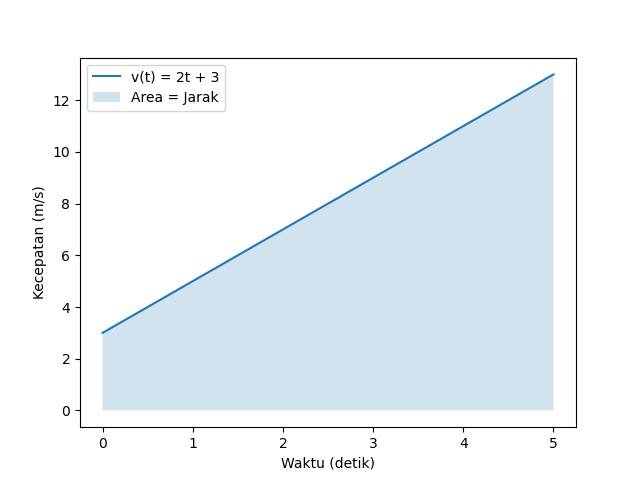
\includegraphics[width=1.01\linewidth]{images/velocity_plot.png}}
\caption{Plot fungsi kecepatan \( v(t) = 2t + 3 \) dan area di bawah kurva yang mewakili jarak tempuh.}
\label{fig:velocity}
\end{figure}

Gambar \ref{fig:velocity} menunjukkan plot fungsi \( v(t) = 2t + 3 \), dengan area di bawah kurva mewakili jarak tempuh. Plot dibuat menggunakan alat visualisasi seperti Python.

\section{Kesimpulan}
Implementasi Aturan Trapesium berhasil menghitung jarak tempuh benda sebesar 40.0000 meter dengan akurasi tinggi (kesalahan relatif 0.000125\%). Metode ini sederhana dan cocok untuk aplikasi teknik. Untuk pengembangan lebih lanjut, metode ini dapat diadaptasi untuk data tabel atau dioptimalkan untuk efisiensi komputasi.

\section{Link}
Kode sumber tersedia di: https://github.com/andrewkristofer/TrapezoidalRule-1 \cite{b2}.

\begin{thebibliography}{00}
\bibitem{b1} S. C. Chapra and R. P. Canale, \textit{Numerical Methods for Engineers}, 7th ed. New York, NY, USA: McGraw-Hill Education, 2015.
\bibitem{b2} Kelompok 1, ``Implementasi Aturan Trapesium untuk Menghitung Jarak Tempuh,'' GitHub, 2025, https://github.com/andrewkristofer/TrapezoidalRule-1.
\end{thebibliography}

\end{document}